\newlength{\figsi}
\setlength{\figsi}{0.9cm} 
\newlength{\figsii}
\setlength{\figsii}{1.8cm} 

\newcommand{\volhighres}[3]{%
\foreach \i in {0, 1, ..., 11} {%
\foreach \j in {0, 1, ..., 7} {%
\pgfmathsetmacro{\dS}{0.5*#3}
\pgfmathsetmacro{\ipo}{\i+1}
\pgfmathsetmacro{\jpo}{\j+1}
\coordinate (p0) at (#1, #2); 
\coordinate (x00) at ($(p0) + (\i*\dS,\j*\dS)$);
\coordinate (x01) at ($(p0) + (\i*\dS,\jpo*\dS)$);
\coordinate (x10) at ($(p0) + (\ipo*\dS,\j*\dS)$);
\coordinate (x11) at ($(p0) + (\ipo*\dS,\jpo*\dS)$);
\draw (x00) -- (x10);
\draw (x00) -- (x01);
\draw (x10) -- (x11);
\draw (x01) -- (x11);
}}
\foreach \i in {0, 1, ..., 8} {%
\foreach \j in {0, 1, ..., 7} {%
\pgfmathsetmacro{\dx}{0.2*#3}
\pgfmathsetmacro{\dy}{0.1*#3}
\pgfmathsetmacro{\dS}{0.5*#3}
\pgfmathsetmacro{\ipo}{\i+1}
\pgfmathsetmacro{\jpo}{\j+1}
\coordinate (p0) at (#1, #2); 
\coordinate (x000) at ($(p0) + (-\i*\dx,\i*\dy+\j*\dS)$); 
\coordinate (x001) at ($(p0) + (-\i*\dx,\i*\dy+\jpo*\dS)$); 
\coordinate (x010) at ($(p0) + (-\ipo*\dx,\ipo*\dy+\j*\dS)$); 
\coordinate (x011) at ($(p0) + (-\ipo*\dx,\ipo*\dy+\jpo*\dS)$); 
\draw (x000) -- (x010);
\draw (x000) -- (x001);
\draw (x010) -- (x011);
\draw (x001) -- (x011);
}}
\foreach \i in {0, 1, ..., 11} {%
\foreach \j in {0, 1, ..., 8} {%
\pgfmathsetmacro{\dx}{0.2*#3}
\pgfmathsetmacro{\dy}{0.1*#3}
\pgfmathsetmacro{\dS}{0.5*#3}
\pgfmathsetmacro{\ipo}{\i+1}
\pgfmathsetmacro{\jpo}{\j+1}
\coordinate (p0) at (#1, #2); 
\coordinate (x800) at ($(p0) + (\i*\dS-\j*\dx,8*\dS+\j*\dy)$); 
\coordinate (x801) at ($(p0) + (\i*\dS-\jpo*\dx,8*\dS+\jpo*\dy)$); 
\coordinate (x810) at ($(p0) + (\ipo*\dS-\j*\dx,8*\dS+\j*\dy)$); 
\coordinate (x811) at ($(p0) + (\ipo*\dS-\jpo*\dx,8*\dS+\jpo*\dy)$); 
\draw (x800) -- (x810);
\draw (x800) -- (x801);
\draw (x810) -- (x811);
\draw (x801) -- (x811);
}}}

\newcommand{\vollowres}[3]{%
\foreach \i in {0, 1, ..., 2} {%
\foreach \j in {0, 1, ..., 1} {%
\pgfmathsetmacro{\dx}{0.8*#3}
\pgfmathsetmacro{\dy}{0.4*#3}
\pgfmathsetmacro{\dS}{2*#3}
\pgfmathsetmacro{\ipo}{\i+1}
\pgfmathsetmacro{\jpo}{\j+1}
\coordinate (p0) at (#1, #2); 
\coordinate (x00) at ($(p0) + (\i*\dS,\j*\dS)$);
\coordinate (x01) at ($(p0) + (\i*\dS,\jpo*\dS)$);
\coordinate (x10) at ($(p0) + (\ipo*\dS,\j*\dS)$);
\coordinate (x11) at ($(p0) + (\ipo*\dS,\jpo*\dS)$);
\draw (x00) -- (x10);
\draw (x00) -- (x01);
\draw (x10) -- (x11);
\draw (x01) -- (x11);
}}
\foreach \i in {0, 1, ..., 1} {%
\foreach \j in {0, 1, ..., 1} {%
\pgfmathsetmacro{\dx}{0.8*#3}
\pgfmathsetmacro{\dy}{0.4*#3}
\pgfmathsetmacro{\dS}{2*#3}
\pgfmathsetmacro{\ipo}{\i+1}
\pgfmathsetmacro{\jpo}{\j+1}
\coordinate (p0) at (#1, #2); 
\coordinate (x000) at ($(p0) + (-\i*\dx,\i*\dy+\j*\dS)$); 
\coordinate (x001) at ($(p0) + (-\i*\dx,\i*\dy+\jpo*\dS)$); 
\coordinate (x010) at ($(p0) + (-\ipo*\dx,\ipo*\dy+\j*\dS)$); 
\coordinate (x011) at ($(p0) + (-\ipo*\dx,\ipo*\dy+\jpo*\dS)$); 
\draw (x000) -- (x010);
\draw (x000) -- (x001);
\draw (x010) -- (x011);
\draw (x001) -- (x011);
}}
\foreach \i in {0, 1, ..., 2} {%
\foreach \j in {0, 1, ..., 1} {%
\pgfmathsetmacro{\dx}{0.8*#3}
\pgfmathsetmacro{\dy}{0.4*#3}
\pgfmathsetmacro{\dS}{2*#3}
\pgfmathsetmacro{\ipo}{\i+1}
\pgfmathsetmacro{\jpo}{\j+1}
\coordinate (p0) at (#1, #2); 
\coordinate (x800) at ($(p0) + (\i*\dS-\j*\dx,2*\dS+\j*\dy)$); 
\coordinate (x801) at ($(p0) + (\i*\dS-\jpo*\dx,2*\dS+\jpo*\dy)$); 
\coordinate (x810) at ($(p0) + (\ipo*\dS-\j*\dx,2*\dS+\j*\dy)$); 
\coordinate (x811) at ($(p0) + (\ipo*\dS-\jpo*\dx,2*\dS+\jpo*\dy)$); 
\draw (x800) -- (x810);
\draw (x800) -- (x801);
\draw (x810) -- (x811);
\draw (x801) -- (x811);
}}}

\newcommand{\cubehighres}[3]{%
\foreach \i in {0, 1, ..., 7} {%
\foreach \j in {0, 1, ..., 7} {%
\pgfmathsetmacro{\dx}{0.2*#3}
\pgfmathsetmacro{\dy}{0.1*#3}
\pgfmathsetmacro{\dS}{0.5*#3}
\pgfmathsetmacro{\ipo}{\i+1}
\pgfmathsetmacro{\jpo}{\j+1}
\coordinate (p0) at (#1, #2); 
\coordinate (x00) at ($(p0) + (\i*\dS,\j*\dS)$);
\coordinate (x01) at ($(p0) + (\i*\dS,\jpo*\dS)$);
\coordinate (x10) at ($(p0) + (\ipo*\dS,\j*\dS)$);
\coordinate (x11) at ($(p0) + (\ipo*\dS,\jpo*\dS)$);
\coordinate (x000) at ($(p0) + (-\i*\dx,\i*\dy+\j*\dS)$); 
\coordinate (x001) at ($(p0) + (-\i*\dx,\i*\dy+\jpo*\dS)$); 
\coordinate (x010) at ($(p0) + (-\ipo*\dx,\ipo*\dy+\j*\dS)$); 
\coordinate (x011) at ($(p0) + (-\ipo*\dx,\ipo*\dy+\jpo*\dS)$); 
\coordinate (x800) at ($(p0) + (\i*\dS-\j*\dx,8*\dS+\j*\dy)$); 
\coordinate (x801) at ($(p0) + (\i*\dS-\jpo*\dx,8*\dS+\jpo*\dy)$); 
\coordinate (x810) at ($(p0) + (\ipo*\dS-\j*\dx,8*\dS+\j*\dy)$); 
\coordinate (x811) at ($(p0) + (\ipo*\dS-\jpo*\dx,8*\dS+\jpo*\dy)$); 
\draw (x00) -- (x10);
\draw (x00) -- (x01);
\draw (x10) -- (x11);
\draw (x01) -- (x11);
\draw (x000) -- (x010);
\draw (x000) -- (x001);
\draw (x010) -- (x011);
\draw (x001) -- (x011);
\draw (x800) -- (x810);
\draw (x800) -- (x801);
\draw (x810) -- (x811);
\draw (x801) -- (x811);
}}}
\newcommand{\cubelowres}[3]{%
\foreach \i in {0, 1, ..., 1} {%
\foreach \j in {0, 1, ..., 1} {%
\pgfmathsetmacro{\dx}{0.8*#3}
\pgfmathsetmacro{\dy}{0.4*#3}
\pgfmathsetmacro{\dS}{2*#3}
\pgfmathsetmacro{\ipo}{\i+1}
\pgfmathsetmacro{\jpo}{\j+1}
\coordinate (p0) at (#1, #2); 
\coordinate (x00) at ($(p0) + (\i*\dS,\j*\dS)$);
\coordinate (x01) at ($(p0) + (\i*\dS,\jpo*\dS)$);
\coordinate (x10) at ($(p0) + (\ipo*\dS,\j*\dS)$);
\coordinate (x11) at ($(p0) + (\ipo*\dS,\jpo*\dS)$);
\coordinate (x000) at ($(p0) + (-\i*\dx,\i*\dy+\j*\dS)$); 
\coordinate (x001) at ($(p0) + (-\i*\dx,\i*\dy+\jpo*\dS)$); 
\coordinate (x010) at ($(p0) + (-\ipo*\dx,\ipo*\dy+\j*\dS)$); 
\coordinate (x011) at ($(p0) + (-\ipo*\dx,\ipo*\dy+\jpo*\dS)$); 
\coordinate (x800) at ($(p0) + (\i*\dS-\j*\dx,2*\dS+\j*\dy)$); 
\coordinate (x801) at ($(p0) + (\i*\dS-\jpo*\dx,2*\dS+\jpo*\dy)$); 
\coordinate (x810) at ($(p0) + (\ipo*\dS-\j*\dx,2*\dS+\j*\dy)$); 
\coordinate (x811) at ($(p0) + (\ipo*\dS-\jpo*\dx,2*\dS+\jpo*\dy)$); 
\draw (x00) -- (x10);
\draw (x00) -- (x01);
\draw (x10) -- (x11);
\draw (x01) -- (x11);
\draw (x000) -- (x010);
\draw (x000) -- (x001);
\draw (x010) -- (x011);
\draw (x001) -- (x011);
\draw (x800) -- (x810);
\draw (x800) -- (x801);
\draw (x810) -- (x811);
\draw (x801) -- (x811);
}}}


\tikzset{figlabel/.style={text centered,font=\bfseries}}
\tikzset{box/.style={text centered,draw,minimum height=2cm}}
\tikzset{boxiii/.style={box,minimum width=3cm,}}
\tikzset{boxiv/.style={box,minimum width=4cm,}}
\tikzset{boxvi/.style={box,minimum width=6cm}}
\tikzset{textciv/.style={text centered,text width=4cm}}
\tikzset{textciii/.style={text centered,text width=3cm}}
\tikzset{textcii/.style={text centered,text width=2cm}}

\newcommand{\figuretemplate}{%
\begin{tikzpicture}[x=1cm,y=1cm]
% \draw [help lines] (0,0) grid (20, 8); 
\pgfmathsetmacro{\dx}{1}
\pgfmathsetmacro{\dy}{1}
\coordinate (p1a) at (1.5, 0); 
\coordinate (p1b) at (1.5, 3.5); 
\coordinate (p1c) at (1.5, 6); 
\coordinate (p2a) at (7, 0.9); 
\coordinate (p2b) at (7, 3.5); 
\coordinate (p2c) at (7, 6); 
\coordinate (p3a) at (14, 0.9); 
\coordinate (p3b) at (14, 3.5);
\coordinate (p3c) at (14, 6);
\coordinate (x00) at (0*\dx,0*\dy); 
\coordinate (x10) at (1*\dx,0*\dy); 
\coordinate (x20) at (2*\dx,0*\dy); 
\coordinate (x30) at (3*\dx,0*\dy); 
\coordinate (x40) at (4*\dx,0*\dy); 
\coordinate (x01) at (0*\dx,1*\dy); 
\coordinate (x11) at (1*\dx,1*\dy); 
\coordinate (x21) at (2*\dx,1*\dy); 
\coordinate (x31) at (3*\dx,1*\dy); 
\coordinate (x41) at (4*\dx,1*\dy); 
\coordinate (x0p2) at (0.5*\dx,2*\dy); 
\coordinate (x1p2) at (1.5*\dx,2*\dy); 
\coordinate (x2p2) at (2.5*\dx,2*\dy); 
\coordinate (x3p2) at (3.5*\dx,2*\dy); 
\coordinate (x4p2) at (4.5*\dx,2*\dy); 
\coordinate (x0p3) at (0.5*\dx,3*\dy); 
\coordinate (x1p3) at (1.5*\dx,3*\dy); 
\coordinate (x2p3) at (2.5*\dx,3*\dy); 
\coordinate (x3p3) at (3.5*\dx,3*\dy); 
\coordinate (x4p3) at (4.5*\dx,3*\dy); 
\coordinate (x02) at (0*\dx,2*\dy); 
\coordinate (x12) at (1*\dx,2*\dy); 
\coordinate (x03) at (0*\dx,3*\dy); 
\coordinate (x13) at (1*\dx,3*\dy); 
\coordinate (x04) at (0*\dx,4*\dy); 
\coordinate (x14) at (1*\dx,4*\dy); 
\coordinate (dec) at (0.5*\dx,0.5*\dy); 
\begin{scope}[xshift=0, yshift=-0.5cm]
\node at ($(dec) + (x11)$) {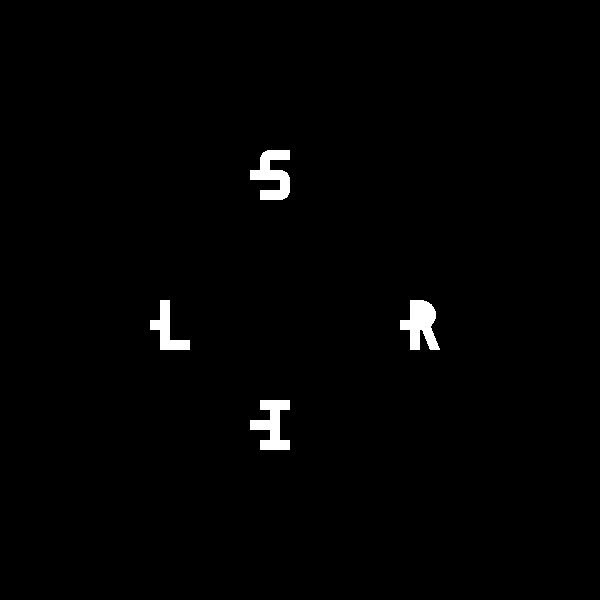
\includegraphics[width=\figsi]{../figs/LRIS.png}};
\node at ($(dec) + (x10)$) {
\includegraphics[width=\figsi]{../figs/LRISbase.png}};
\node at ($(dec) + (x21)$) {
\includegraphics[width=\figsi]{../figs/LRPA.png}};
\node at ($(dec) + (x20)$) {
\includegraphics[width=\figsi]{../figs/LRPAbase.png}};
\node at ($(dec) + (x01)$) {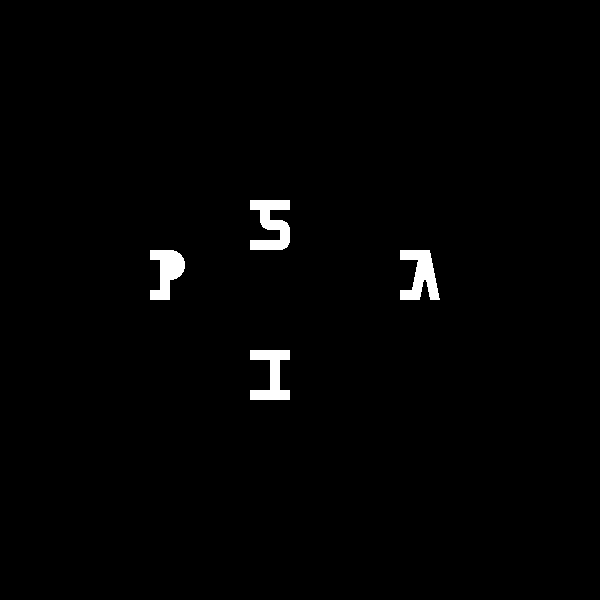
\includegraphics[width=\figsi]{../figs/PAIS.png}};
\node at ($(dec) + (x00)$) {
\includegraphics[width=\figsi]{../figs/PAISbase.png}};
\node at ($(dec) + (x0p3)$) {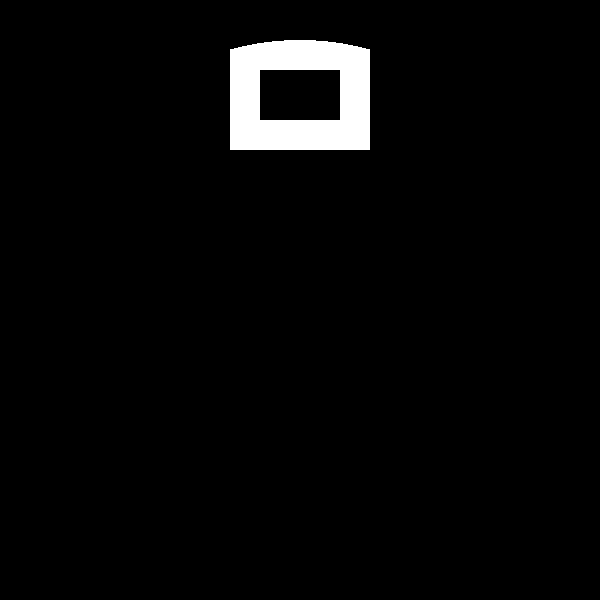
\includegraphics[width=\figsi]{../figs/maintainer1.png}};
\node at ($(dec) + (x0p2)$) {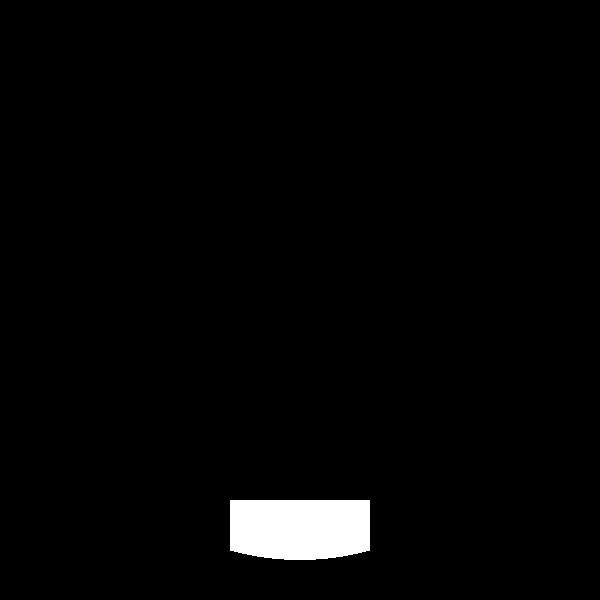
\includegraphics[width=\figsi]{../figs/maintainer2.png}};
\node at ($(dec) + (x1p3)$) {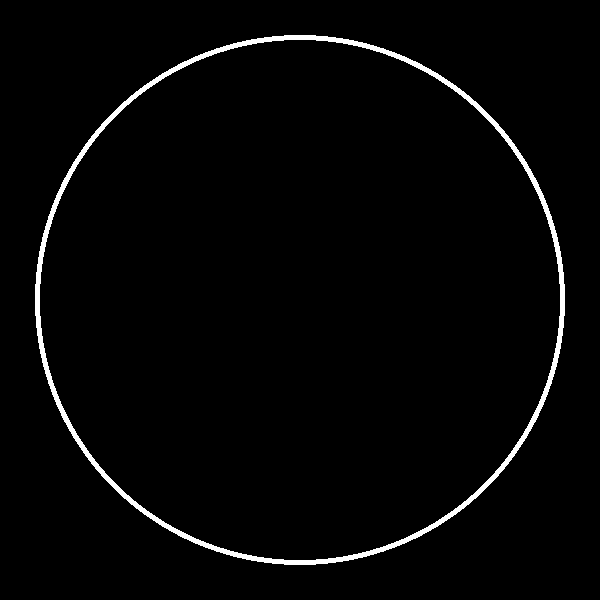
\includegraphics[width=\figsi]{../figs/tube.png}};
\node at ($(dec) + (x1p2)$) {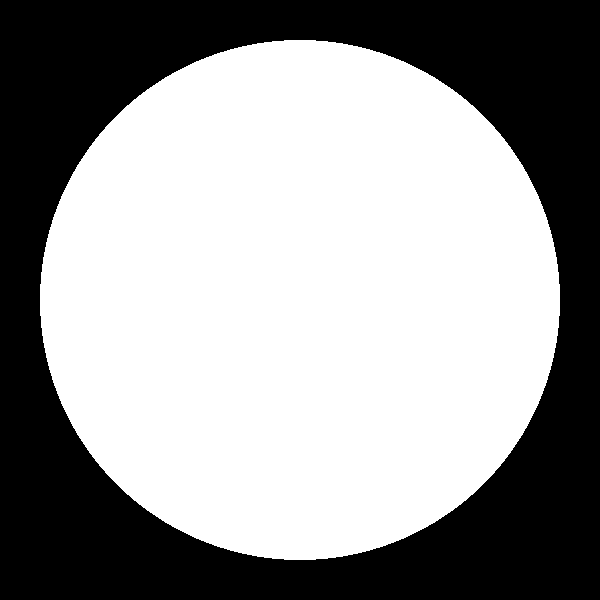
\includegraphics[width=\figsi]{../figs/water.png}};
\end{scope}
\cubehighres{5}{5.5}{0.2}
\node  at (p2a) {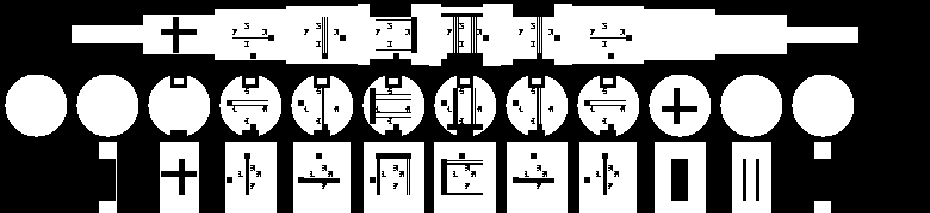
\includegraphics[width=6cm]{../figs/template-mri_resolution-0100.png}};
\node  at (p2b) {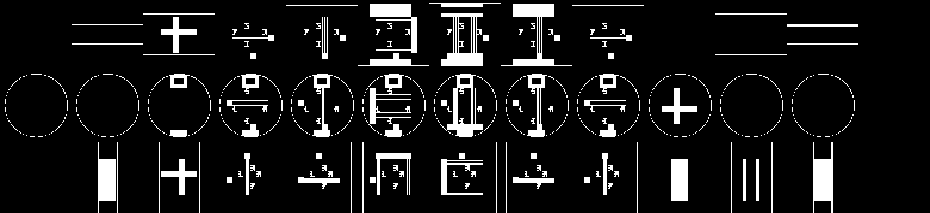
\includegraphics[width=6cm]{../figs/template-ct_resolution-0100.png}};
\node [yshift=1.2cm] at (p2a) {MRI}; 
\node [yshift=1.2cm] at (p2b) {CT}; 
\cubelowres{12}{5.5}{0.2}
\node at (p3a) {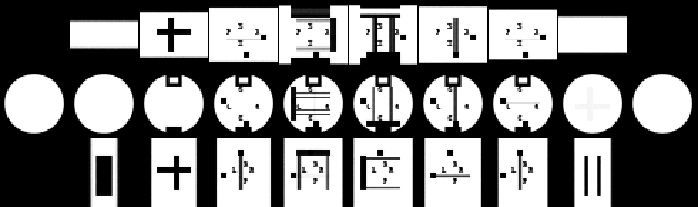
\includegraphics[width=6cm]{../figs/template-mri_resolution-1250.png}};
\node at (p3b) {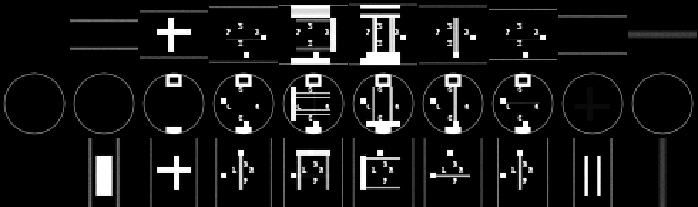
\includegraphics[width=6cm]{../figs/template-ct_resolution-1250.png}};
\node [yshift=1.2cm] at (p3a) {MRI}; 
\node [yshift=1.2cm] at (p3b) {CT}; 
\node [boxiii] (b1) at (p1c) {}; 
\node [boxvi] (b2) at (p2c) {}; 
\node [boxvi] (b3) at (p3c) {}; 
\node [textciii] at (p1c) {High-Resolution Masks and Geometric Shapes (0.100 mm)}; 
\node [textciv, xshift=0.8cm] at (p2c) {High-Resolution\\ Template (0.100 mm)}; 
\node [textciv, xshift=0.8cm] at (p3c) {Low-Resolution\\ Template (1.250 mm)}; 
\draw [->,>=latex] (b1) -- (b2); 
\draw [->,>=latex] (b2) -- (b3); 
\node [figlabel,yshift=0.5cm] at (b1.north) {a}; 
\node [figlabel,yshift=0.5cm] at (b2.north) {b}; 
\node [figlabel,yshift=0.5cm] at (b3.north) {c}; 
\end{tikzpicture}
}

\newcommand{\figurealign}{%
\begin{tikzpicture}[x=1cm,y=1cm]
%\draw [help lines] (0, 0) grid (20, 10);
\coordinate (p1) at (2.5, 6); 
\coordinate (p2) at (8, 6); 
\coordinate (p3) at (2.5, 1.5); 
\coordinate (p4) at (8, 1.5); 
\coordinate (p5) at (12.25, 6); 
\coordinate (p6) at (12.25, 1.5); 
\coordinate (p7) at (14.75, 6); 
\coordinate (p8) at (17, 6); 

\node [boxiv,minimum width=5cm,minimum height=3cm] (b1) at (p1) {}; 
\cubelowres{0.75}{6.25}{0.2}
\node [textciii,xshift=1cm,yshift=0.75cm] at (p1) {Low-Resolution Template}; 
\node [yshift=-0.75cm] at (p1) {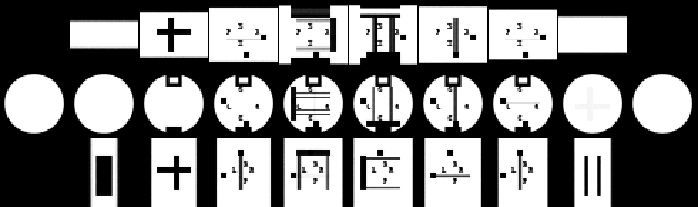
\includegraphics[width=4cm]{../figs/template-mri_resolution-1250.png}};
% block 2 -- flips and permutations
\node [minimum width=5.5cm,minimum height=5cm,draw] (b2) at (p2) {};
\node [textciv, yshift=2cm] at (b2) {Flips and Permutations}; 
\node [xshift=-0.2cm,yshift=-0.35cm] at (p2) {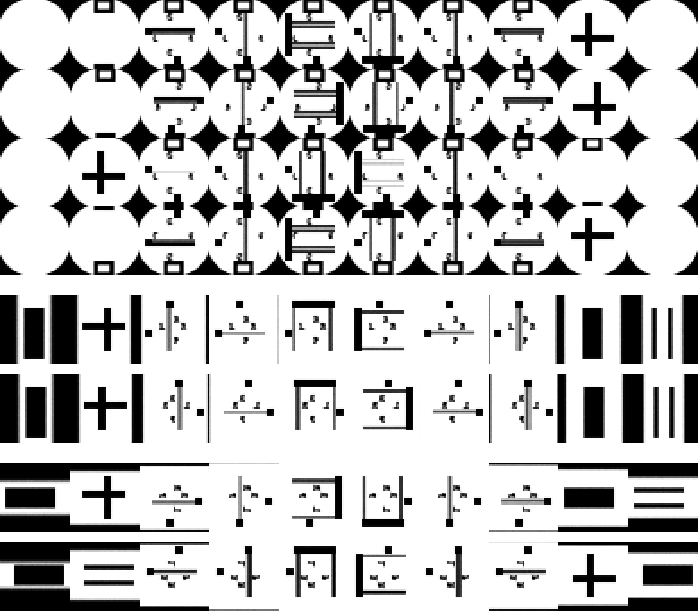
\includegraphics[width=4cm]{../figs/patterns.png}}; 
\node [xshift=-2.3cm, yshift=1.15cm] (W21l) at (p2) {}; 
\node [xshift=-2.3cm, yshift=0.75cm] (W22l) at (p2) {};
\node [xshift=-2.3cm, yshift=0cm] (W2ll) at (p2) {};
\node [xshift=-2.3cm, yshift=-1.95cm] (W2Nl) at (p2) {};
\node [xshift=2.3cm, yshift=1.15cm] (W21r) at (p2) {$W_1$}; 
\node [xshift=2.3cm, yshift=0.75cm] (W22r) at (p2) {$W_2$};
\node [xshift=2.3cm, yshift=0cm] (W2lr) at (p2) {$W_l$};
\node [xshift=2.3cm, yshift=-1.95cm] (W2Nr) at (p2) {$W_N$};
% block 3 -- vol high res 
\node [draw,minimum width=5cm,minimum height=3cm] (b3) at (p3) {}; 
\volhighres{0.75}{1.5}{0.2}
\node [textciii,xshift=1cm,yshift=0.75cm] at (p3) {High-Resolution Volume}; 
\node [yshift=-0.75cm] at (p3) {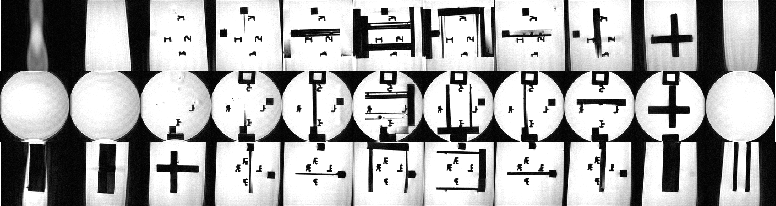
\includegraphics[width=4cm]{../figs/sub-1_ses-1_resolution-0391.png}};
% block 4 -- vol low res
\node [draw,minimum width=5cm,minimum height=3cm] (b4) at (p4) {}; 
\vollowres{6.5}{1.5}{0.2}
\node [textciii,xshift=1cm,yshift=0.75cm] at (p4) {Low-Resolution Volume \& Cropping}; 
\node [yshift=-0.75cm] at (p4) {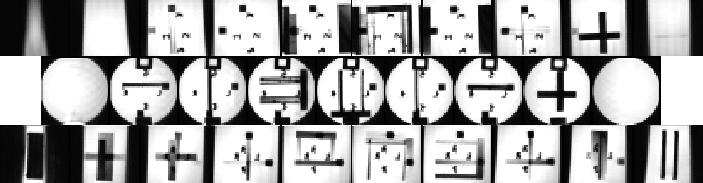
\includegraphics[width=4cm]{../figs/sub-1_ses-1_resolution-1250.png}};
% block 5 -- flatten and translations
\node [draw,minimum width=2.5cm,minimum height=5cm] (b5) at (p5) {}; 
\node [textcii, yshift=2cm] at (p5) {Translations \\ \& Flattening}; 
\node [textcii] at (p5) {$W_{l, \tau}$}; 
% \node [textcii, yshift=-1cm] at (p5) {\small $\tau = (\tau_i, \tau_j, \tau_k)$}; 
%    figure flatten 1
\path (p5) -- ++(-0.75,+1.05) node [coordinate] (i0) {};
\draw [fill=black] (i0) -- ++(0.2,0) -- ++(0,0.2) -- ++(-0.2,0) --cycle; 
\path (i0) -- ++(0.2,0) node [coordinate] (i) {};
\draw [fill=gray] (i) -- ++(0.2,0) -- ++(0,0.2) -- ++(-0.2,0) --cycle; 
\path (i0) -- ++(0.4,0) node [coordinate] (i) {};
\draw [fill=black] (i) -- ++(0.2,0) -- ++(0,0.2) -- ++(-0.2,0) --cycle; 
\path (i0) -- ++(0.6,0) node [coordinate] (i) {};
\draw [dotted] (i) -- ++(0.5,0); 
\path (i0) -- ++(0.6,0.2) node [coordinate] (i) {};
\draw [dotted] (i) -- ++(0.5,0); 
\path (i0) -- ++(1.1,0) node [coordinate] (i) {};
\draw [fill=white] (i) -- ++(0.2,0) -- ++(0,0.2) -- ++(-0.2,0) --cycle; 
\path (i0) -- ++(1.3,0) node [coordinate] (i) {};
\draw [fill=white] (i) -- ++(0.2,0) -- ++(0,0.2) -- ++(-0.2,0) --cycle; 
%    figure flatten 2
\path (p5) -- ++(-0.75,+0.8) node [coordinate] (i0) {};
\draw [fill=white] (i0) -- ++(0.2,0) -- ++(0,0.2) -- ++(-0.2,0) --cycle; 
\path (i0) -- ++(0.2,0) node [coordinate] (i) {};
\draw [fill=black] (i) -- ++(0.2,0) -- ++(0,0.2) -- ++(-0.2,0) --cycle; 
\path (i0) -- ++(0.4,0) node [coordinate] (i) {};
\draw [fill=gray] (i) -- ++(0.2,0) -- ++(0,0.2) -- ++(-0.2,0) --cycle; 
\path (i0) -- ++(0.6,0) node [coordinate] (i) {};
\draw [dotted] (i) -- ++(0.5,0); 
\path (i0) -- ++(0.6,0.2) node [coordinate] (i) {};
\draw [dotted] (i) -- ++(0.5,0); 
\path (i0) -- ++(1.1,0) node [coordinate] (i) {};
\draw [fill=gray] (i) -- ++(0.2,0) -- ++(0,0.2) -- ++(-0.2,0) --cycle; 
\path (i0) -- ++(1.3,0) node [coordinate] (i) {};
\draw [fill=white] (i) -- ++(0.2,0) -- ++(0,0.2) -- ++(-0.2,0) --cycle; 
%    connectors
\node [xshift=-0.9cm, yshift=1.15cm] (W511l) at (p5) {}; 
\node [xshift=-0.9cm, yshift=1.05cm] (W512l) at (p5) {}; 
\node [xshift=-0.9cm, yshift=0.9cm] (W513l) at (p5) {}; 
\node [xshift=-0.9cm, yshift=0.75cm] (W521l) at (p5) {};
\node [xshift=-0.9cm, yshift=0cm] (W5l1l) at (p5) {};
\node [xshift=-0.9cm, yshift=-1.95cm] (W5N1l) at (p5) {};
\node [xshift=0.9cm, yshift=1.15cm] (W511r) at (p5) {}; 
\node [xshift=0.9cm, yshift=1.05cm] (W512r) at (p5) {}; 
\node [xshift=0.9cm, yshift=0.9cm] (W51kr) at (p5) {}; 
\node [xshift=0.9cm, yshift=0.75cm] (W521r) at (p5) {};
\node [xshift=0.9cm, yshift=0.7cm] (W522r) at (p5) {};
\node [xshift=0.9cm, yshift=0.6cm] (W52kr) at (p5) {};
\node [xshift=0.9cm, yshift=0cm] (W5l1r) at (p5) {};
\node [xshift=0.9cm, yshift=-0.1cm] (W5l2r) at (p5) {};
\node [xshift=0.9cm, yshift=-0.3cm] (W5lkr) at (p5) {};
\node [xshift=0.9cm, yshift=-1.95cm] (W5N1r) at (p5) {};
\node [xshift=0.9cm, yshift=-2.0cm] (W5N2r) at (p5) {};
\node [xshift=0.9cm, yshift=-2.2cm] (W5Nkr) at (p5) {};
% block 6 -- flatten
\node [draw,minimum width=2.5cm,minimum height=3cm] (b6) at (p6) {}; 
\node [textciii, yshift=0.75cm] at (p6) {Flattening}; 
\node [yshift=0cm] (X) at (p6) {X};
%    figure flatten volume
\path (p6) -- ++(-0.75,-0.75) node [coordinate] (i0) {};
\draw [fill=white] (i0) -- ++(0.2,0) -- ++(0,0.2) -- ++(-0.2,0) --cycle; 
\path (i0) -- ++(0.2,0) node [coordinate] (i) {};
\draw [fill=black] (i) -- ++(0.2,0) -- ++(0,0.2) -- ++(-0.2,0) --cycle; 
\path (i0) -- ++(0.4,0) node [coordinate] (i) {};
\draw [fill=gray] (i) -- ++(0.2,0) -- ++(0,0.2) -- ++(-0.2,0) --cycle; 
\path (i0) -- ++(0.6,0) node [coordinate] (i) {};
\draw [dotted] (i) -- ++(0.5,0); 
\path (i0) -- ++(0.6,0.2) node [coordinate] (i) {};
\draw [dotted] (i) -- ++(0.5,0); 
\path (i0) -- ++(1.1,0) node [coordinate] (i) {};
\draw [fill=gray] (i) -- ++(0.2,0) -- ++(0,0.2) -- ++(-0.2,0) --cycle; 
\path (i0) -- ++(1.3,0) node [coordinate] (i) {};
\draw [fill=white] (i) -- ++(0.2,0) -- ++(0,0.2) -- ++(-0.2,0) --cycle; 
% block 7 -- score
\node [draw,minimum width=2cm,minimum height=5cm] (b7) at (p7) {}; 
\node [textciii,yshift=2cm] at (p7) {Score\\ Evaluation}; 
\node (Sj) at (p7) {$S_{l,\tau}$}; 
\node [yshift=-1cm] at (p7) {\small $ = \frac{W_{l,\tau}^T \, X}{||W_1||\,||X||}$}; 
\node [xshift=-0.7cm, yshift=1.15cm] (W711l) at (p7) {}; 
\node [xshift=-0.7cm, yshift=1.05cm] (W712l) at (p7) {}; 
\node [xshift=-0.7cm, yshift=0.9cm] (W71kl) at (p7) {}; 
\node [xshift=-0.7cm, yshift=0.75cm] (W721l) at (p7) {};
\node [xshift=-0.7cm, yshift=0.7cm] (W722l) at (p7) {};
\node [xshift=-0.7cm, yshift=0.5cm] (W72kl) at (p7) {};
\node [xshift=-0.7cm, yshift=0cm] (W7l1l) at (p7) {};
\node [xshift=-0.7cm, yshift=-0.2cm] (W7l2l) at (p7) {};
\node [xshift=-0.7cm, yshift=-0.4cm] (W7lkl) at (p7) {};
\node [xshift=-0.7cm, yshift=-1.95cm] (W7N1l) at (p7) {};
\node [xshift=-0.7cm, yshift=-2cm] (W7N2l) at (p7) {};
\node [xshift=-0.7cm, yshift=-2.2cm] (W7Nkl) at (p7) {};
\node [xshift=0.7cm, yshift=1.15cm] (W711r) at (p7) {}; 
\node [xshift=0.7cm, yshift=1.05cm] (W712r) at (p7) {}; 
\node [xshift=0.7cm, yshift=0.9cm] (W71kr) at (p7) {}; 
\node [xshift=0.7cm, yshift=0.75cm] (W721r) at (p7) {};
\node [xshift=0.7cm, yshift=0.7cm] (W722r) at (p7) {};
\node [xshift=0.7cm, yshift=0.6cm] (W72kr) at (p7) {};
\node [xshift=0.7cm, yshift=0cm] (W7l1r) at (p7) {};
\node [xshift=0.7cm, yshift=-0.2cm] (W7l2r) at (p7) {};
\node [xshift=0.7cm, yshift=-0.4cm] (W7lkr) at (p7) {};
\node [xshift=0.7cm, yshift=-1.95cm] (W7N1r) at (p7) {};
\node [xshift=0.7cm, yshift=-2cm] (W7N2r) at (p7) {};
\node [xshift=0.7cm, yshift=-2.2cm] (W7Nkr) at (p7) {};
% block 8 -- max fit
\node [draw,minimum width=2cm,minimum height=5cm] (b8) at (p8) {}; 
\node [textciii,yshift=2cm] at (p8) {Best Fit\\ Selection}; 
\node at (p8) {$(l^*, \tau^*)$}; 
\node [yshift=-0.75cm] at (p8) {\small $=$}; 
\node [yshift=-1cm] at (p8) {\small $\arg\max S_{l, \tau}$}; 
\node [yshift=-1.25cm] at (p8) {\scriptsize $(l,\tau) \in \mathcal{L}\times\mathcal{T}$}; 
\node [xshift=-0.7cm, yshift=1.15cm] (W811l) at (p8) {}; 
\node [xshift=-0.7cm, yshift=1.05cm] (W812l) at (p8) {}; 
\node [xshift=-0.7cm, yshift=0.9cm] (W81kl) at (p8) {}; 
\node [xshift=-0.7cm, yshift=0.75cm] (W821l) at (p8) {};
\node [xshift=-0.7cm, yshift=0.7cm] (W822l) at (p8) {};
\node [xshift=-0.7cm, yshift=0.5cm] (W82kl) at (p8) {};
\node [xshift=-0.7cm, yshift=0cm] (W8l1l) at (p8) {};
\node [xshift=-0.7cm, yshift=-0.2cm] (W8l2l) at (p8) {};
\node [xshift=-0.7cm, yshift=-0.4cm] (W8lkl) at (p8) {};
\node [xshift=-0.7cm, yshift=-1.95cm] (W8N1l) at (p8) {};
\node [xshift=-0.7cm, yshift=-2cm] (W8N2l) at (p8) {};
\node [xshift=-0.7cm, yshift=-2.2cm] (W8Nkl) at (p8) {};
% connections
\draw [->,>=latex] (b1.east) -- (W21l.west); 
\draw [->,>=latex] (b1.east) -- (W22l.west); 
\draw [->,>=latex] (b1.east) -- (W2Nl.west); 
% \draw [->,>=latex] (b1.east) -- (b2.west); 
\draw [->,>=latex] (b3.east) -- (b4.west);
\draw [->,>=latex] (b4.east) -- (X.west); 
\draw [->,>=latex] (X.east) -| (b7.south); 
% \draw [->,>=latex] (Sj.east) -- (b8.west); 
\draw [->,>=latex] (W21r) -- (W511l); 
%\draw [->,>=latex] (W21r) -- (W512l); 
\draw [->,>=latex] (W21r) -- (W513l); 
\draw [->,>=latex] (W22r) -- (W521l); 
\draw [->,>=latex] (W2lr) -- (W5l1l); 
\draw [->,>=latex] (W2Nr) -- (W5N1l); 
\draw [->,>=latex] (W511r) -- (W711l); 
%\draw [->,>=latex] (W512r) -- (W712l); 
\draw [->,>=latex] (W51kr) -- (W71kl); 
\draw [->,>=latex] (W521r) -- (W721l); 
%\draw [->,>=latex] (W522r) -- (W722l); 
%\draw [->,>=latex] (W52kr) -- (W72kl); 
\draw [->,>=latex] (W5l1r) -- (W7l1l); 
%\draw [->,>=latex] (W5l2r) -- (W7l2l); 
%\draw [->,>=latex] (W5lkr) -- (W7lkl); 
\draw [->,>=latex] (W5N1r) -- (W7N1l); 
%\draw [->,>=latex] (W5N2r) -- (W7N2l); 
%\draw [->,>=latex] (W5Nkr) -- (W7Nkl); 
\draw [->,>=latex] (W711r) -- (W811l); 
%\draw [->,>=latex] (W712r) -- (W812l); 
\draw [->,>=latex] (W71kr) -- (W81kl); 
\draw [->,>=latex] (W721r) -- (W821l); 
%\draw [->,>=latex] (W722r) -- (W822l); 
%\draw [->,>=latex] (W72kr) -- (W82kl); 
\draw [->,>=latex] (W7l1r) -- (W8l1l); 
% \draw [->,>=latex] (W7l2r) -- (W8l2l); 
%\draw [->,>=latex] (W7lkr) -- (W8lkl); 
\draw [->,>=latex] (W7N1r) -- (W8N1l); 
%\draw [->,>=latex] (W7N2r) -- (W8N2l); 
%\draw [->,>=latex] (W7Nkr) -- (W8Nkl); 
% fig labels
\node [figlabel,yshift=1.75cm] at (p1) {a}; 
\node [figlabel,yshift=2.75cm] at (p2) {b}; 
\node [figlabel,yshift=1.75cm] at (p3) {c}; 
\node [figlabel,yshift=1.75cm] at (p4) {d}; 
\node [figlabel,yshift=2.75cm] at (p5) {e}; 
\node [figlabel,yshift=1.75cm] at (p6) {f}; 
\node [figlabel,yshift=2.75cm] at (p7) {g}; 
\node [figlabel,yshift=2.75cm] at (p8) {h}; 
\end{tikzpicture}
}
